\section{Обзор существующих решений}
\label{sec:Chapter2} \index{Chapter2}
\subsection{Поиск данных в поисковых сервисах}
\subsubsection{Google Dorks (Google Hacking)}
Google Dorks\footnote{https://www.google.com/} - это по сути та же самая поисковая система от Google. Отличие заключается
только в том, что обычный пользователь вбивает типовые запросы а-ля "Какая погода в Москве?", то Google Dorks позволяет
использовать специальные запросы для получения конкрентной информации. Google Dorks имеет множество операторов, которые 
можно использовать для составления очень гибких и точных запросов \cite{googleHackingWikipedia}. По факту, это запросы, с помощью которых можно проверить
безопасность того или иного сайта, найти IP-адреса сервисов, камер. Весьма эффективна для поиска документации по ключевым словам, 
а также поиску людей с помощью тех же самых Google Dorks Queries. 

\parПлюсы данный системы:
\begin{itemize}
    \item быстрый и объемный поиск по ключевым словам.
\end{itemize}

\parИз недостатков системы можно определить следующее:
\begin{itemize}
    \item составленный запрос выдаст перечень ссылок в интерфейсе поисковой системы, а не сами данные;
    \item перед использованием необоходимо изучить синтаксис запросов;
    \item нет накопления собранной информации, нельзя отслеживать изменения (дельты);
    \item нет построения графа зависимостей объекта.
\end{itemize}

\begin{figure}[H]
    \center{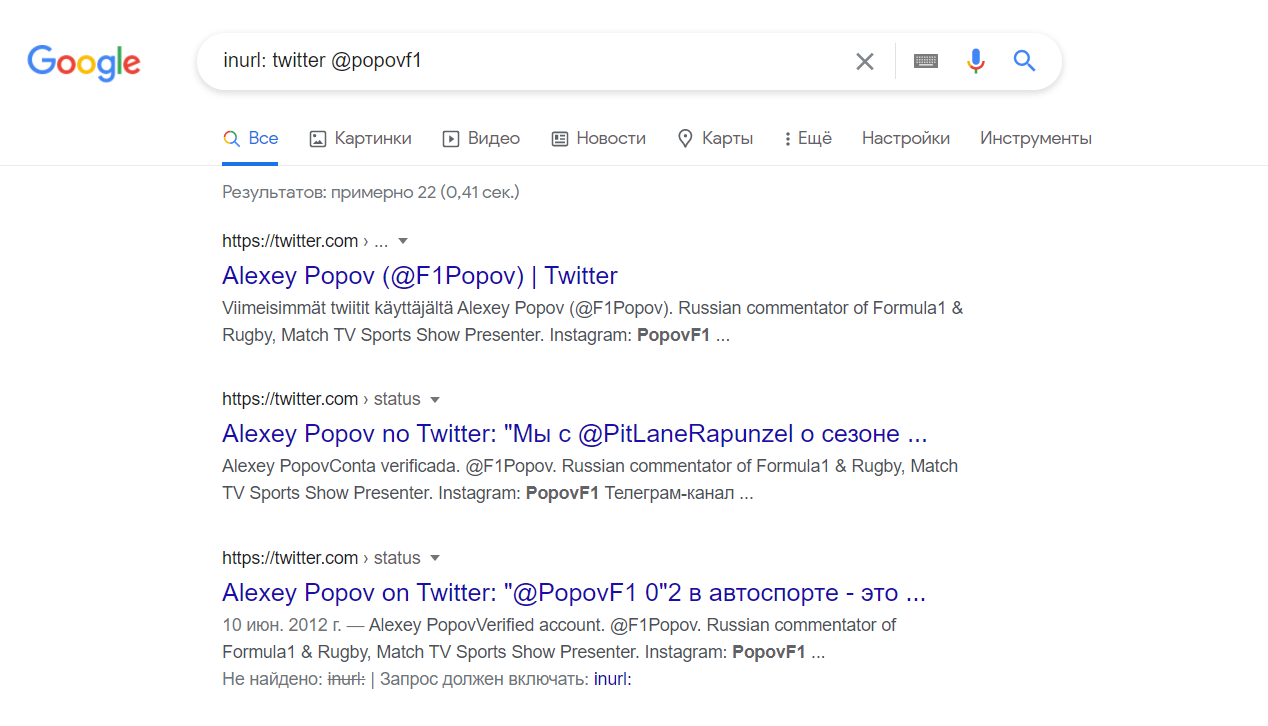
\includegraphics[height=6cm,keepaspectratio]{pictures/GoogleDorksTwitter.png}}
    \caption{Пример использования GDQ для поиска человека.}
    \label{ris:image}
\end{figure}

\subsubsection{Carrot2}
Carrot2 - движок кластеризации результатов поисковых запросов с открытым исходным кодом. Carrot2 может самостоятельно
группировать по категориям найденные документы или данные. Работает в свою очередь как обычный поисковик, то есть
по указанному ключевому слову возвращает некоторое множество ссылок, затем которые группируются по категориям 
\cite{carrot2wikipedia}.

\par
Преимущества:
\begin{itemize}
    \item быстрый и обширный поиск по ключевым словам;
    \item автоматическая группировка данных в соответствии с категориями;
    \item наличие удобного интерфейса с возможностью просмотра древовидной карты и круговидной диаграммы.
\end{itemize}

\par
Недостатки:
\begin{itemize}
    \item как и в случае с Google Dorks, Carrot2 возвращает нам перечень ссылок на источники данных, а не сами данные
     непосредственно;
    \item невозможно произвести точечный поиск файлов и данных, как это реализовано в Google Dorks. Как следствие - 
    большое количество лишней информации.
\end{itemize}


\begin{figure}[H]
    \center{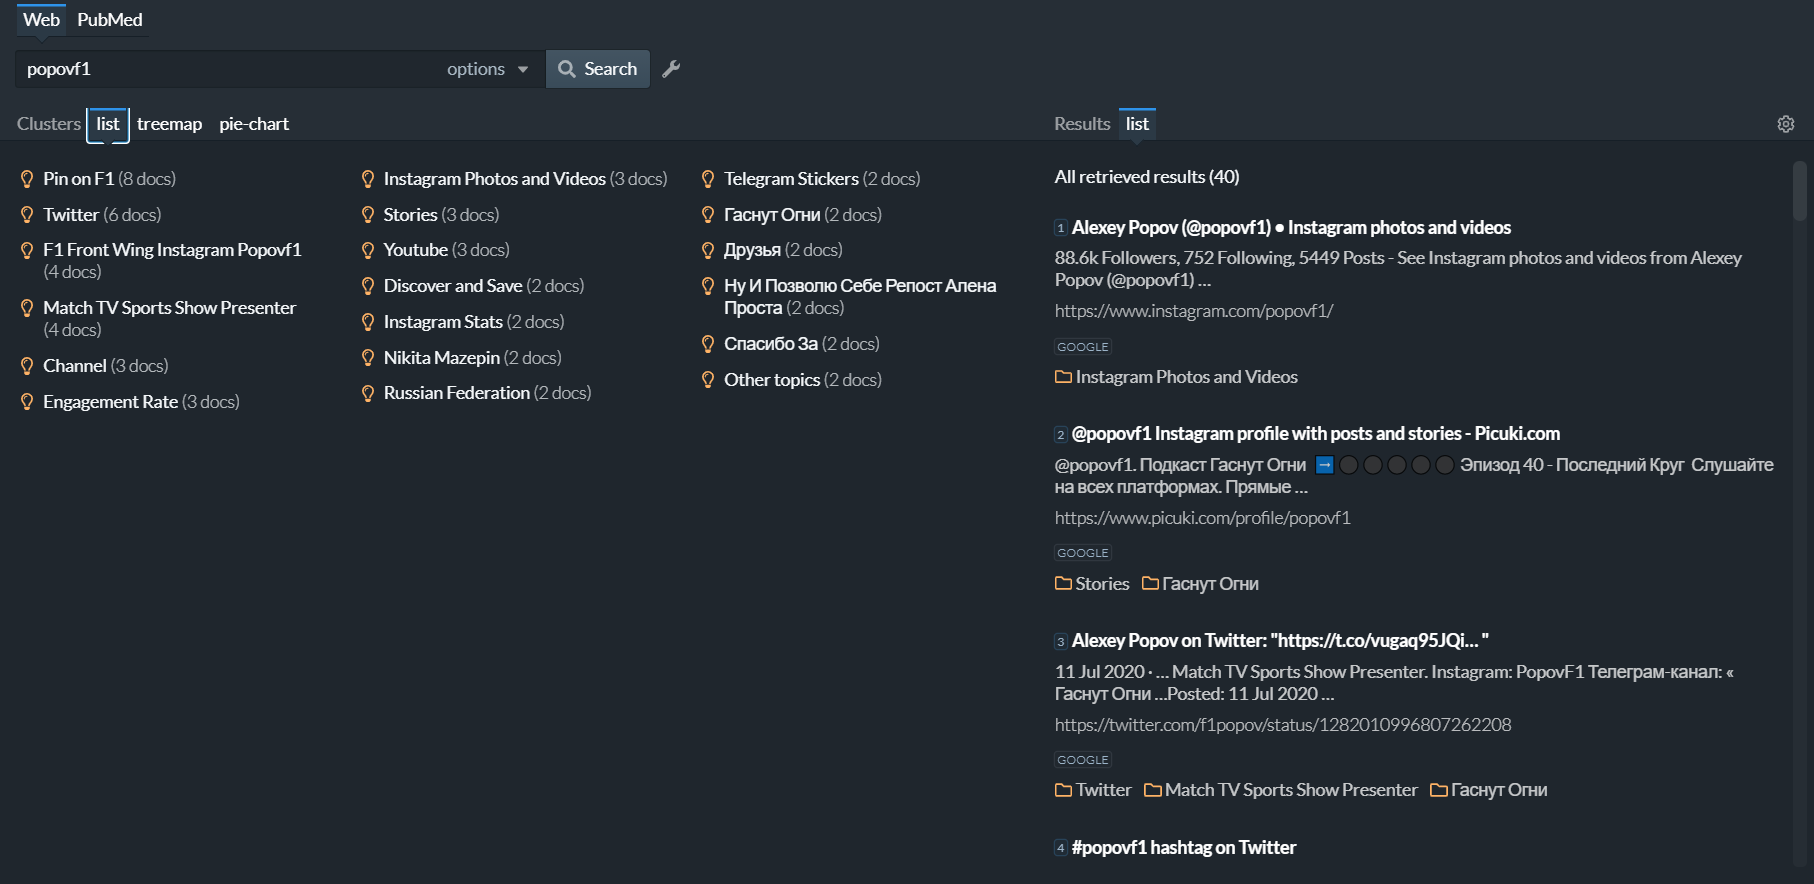
\includegraphics[height=6cm,keepaspectratio]{pictures/Carrot2_1.png}}
    \caption{Пример использования Carrot2 с разбиением результатов на группы.}
    \label{ris:image}
\end{figure}


\subsubsection{Yippy}
Yippy\footnote{http://yippy.com/} - это метапоисковый движок, который группирует результаты поиска на категориям в группы.
Наделен обширным функционалом: позволяет искать по ключевым словам новости, вакансии, правительственную информацию и блоги.
Также позволяет вручную настраивать источники данных для собственного уникального метапоиска. \cite{yippywikipedia}

Преимущества:
\begin{itemize}
    \item группирует данные по тематическим категориям;
    \item есть возможность поиска не только ссылок в web-пространстве, но и непосредственно новостей, изображений и видео;
\end{itemize}

Недостатки:
\begin{itemize}
    \item сервис недоступен на территории РФ;
    \item нет поддержки GDQ.
\end{itemize}

\begin{figure}[H]
    \center{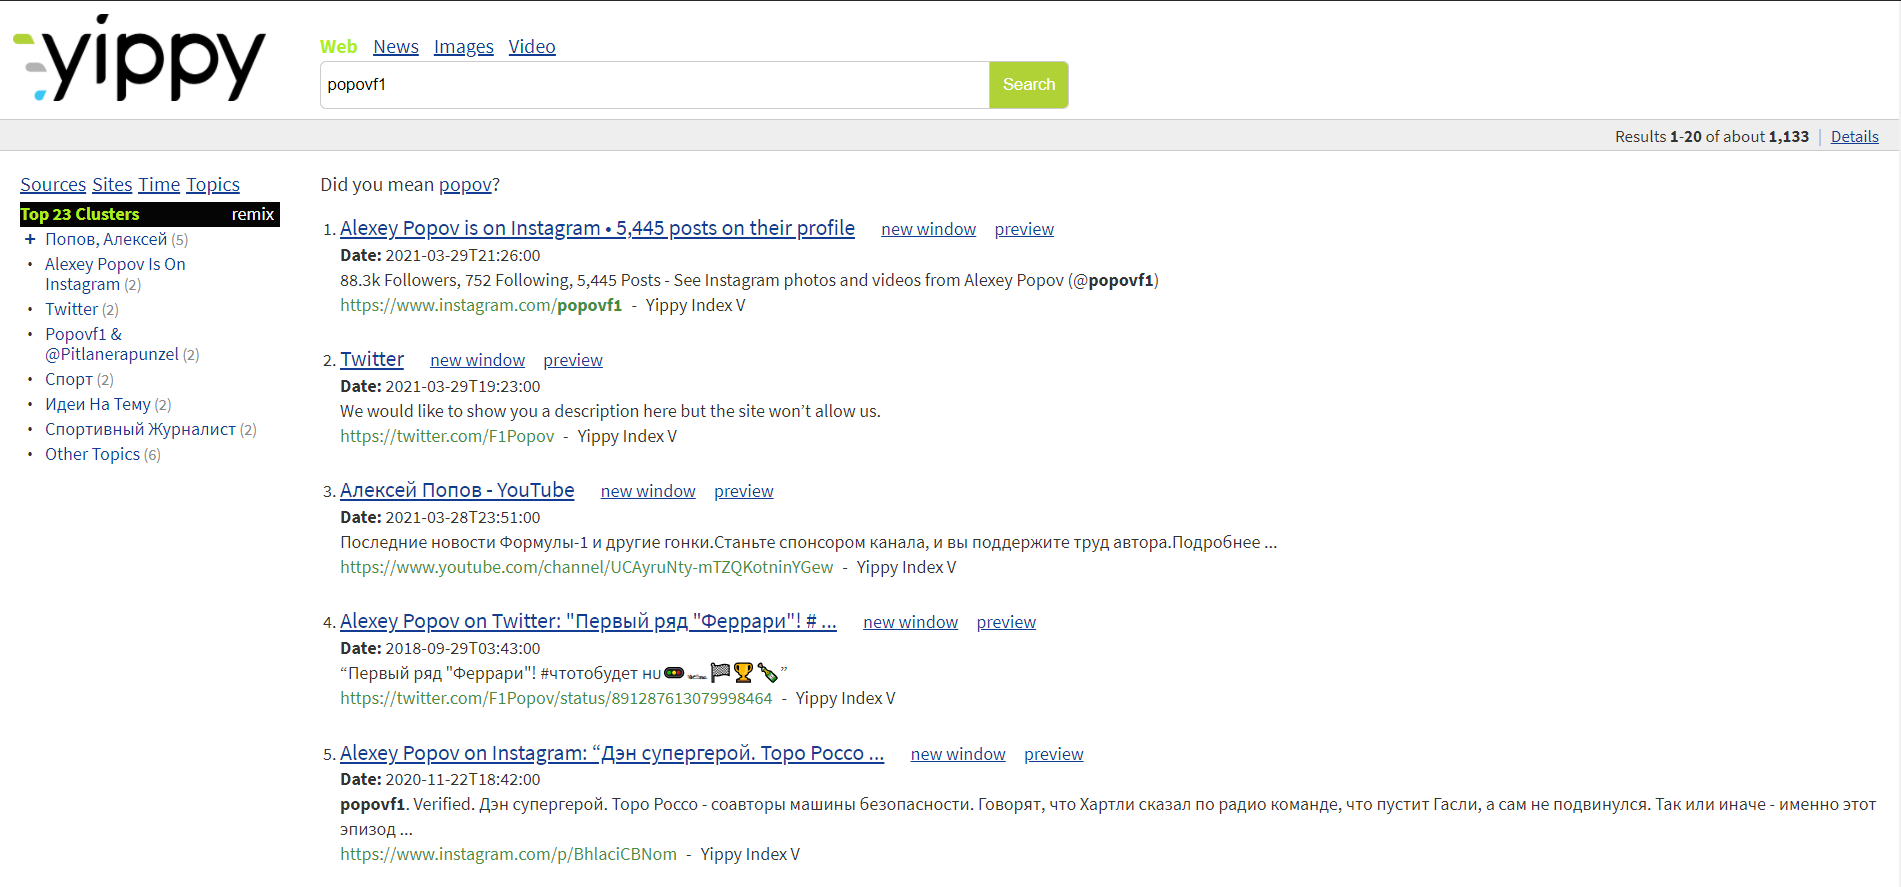
\includegraphics[height=6cm,keepaspectratio]{pictures/yippy_1.png}}
    \caption{Пример использования Yippy.}
    \label{ris:image}
\end{figure}

\subsection{Поиск данных в социальных сетях}
\subsubsection{Maltego}
Maltego\footnote{https://www.maltego.com/} - это


\subsubsection{ITools}
ITools\footnote{http://itools.com/search/people-search} - это


\subsubsection{FindThatLead}
FindThatLead\footnote{https://findthatlead.com/en} - это


\subsubsection{Palantir}
Palantir\footnote{https://www.palantir.com/solutions/intelligence/} - это

\subsection{Универсальные приложения}
\subsubsection{Виток OSINT}
Виток OSINT\footnote{https://norsi-trans.ru/catalog/vitok-osint/} - это
